% Created 2019-07-03 Wed 17:37
% Intended LaTeX compiler: pdflatex
\documentclass[11pt]{article}
\usepackage[utf8]{inputenc}
\usepackage[T1]{fontenc}
\usepackage{graphicx}
\usepackage{grffile}
\usepackage{longtable}
\usepackage{wrapfig}
\usepackage{rotating}
\usepackage[normalem]{ulem}
\usepackage{amsmath}
\usepackage{textcomp}
\usepackage{amssymb}
\usepackage{capt-of}
\usepackage{hyperref}
\usepackage{minted}
\author{Nicolás Luarte}
\date{\today}
\title{Eduardo}
\hypersetup{
 pdfauthor={Nicolás Luarte},
 pdftitle={Eduardo},
 pdfkeywords={},
 pdfsubject={},
 pdfcreator={Emacs 25.2.2 (Org mode 9.2.3)}, 
 pdflang={English}}
\begin{document}

\maketitle
\tableofcontents

\section{Ciclos}
\label{sec:org898bb05}
\subsection{Ciclo 1 (descarga):}
\label{sec:org150445f}
\begin{center}
\begin{tabular}{lll}
Ejercicio & Protocolo & Bloque\\
Sentadilla beltless & x6@ 7, 8, 9 & A\\
Bus drivers & x10@ 7,8,9 -5\% 1x10 & A\\
Bird dog & 4x10 (10 por lado) & A\\
RKC plank & 4x todo el tiempo posible & A\\
One handed barbell row & 15@7, 8, 9 -5\% 1x15 & A\\
\hline
Press banca pies arriba & x6@ 7, 8, 9 & B\\
Pull ups & 3x10 & B\\
Biceps curl & 3x15 & B\\
Buenos días & 3x8 & B\\
RKC planks & 3x todo el tiempo posible & B\\
\hline
Peso muerto competencia & x6@ 7, 8, 9 & C\\
RKC planks & 3x todo el tiempo posible & C\\
Side planks & 2x 1 minuto (por lado) & C\\
Bird dog & 3x10 (por lado) & C\\
Crunches & 3x todos los posible & C\\
\hline
RKC planks & 4x todo el tiempo posible & D\\
Side planks & 2x 1 minuto (por lado) & D\\
RKC planks & 2x todo el tiempo posible & D\\
Rodillas al pecho colgando (abs) & 3xamrap & D\\
 &  & \\
\end{tabular}
\end{center}

\subsubsection{Links}
\label{sec:org705dd3b}
\subsubsection{Bus drivers}
\label{sec:org0f06946}
\url{https://www.youtube.com/watch?v=xDvNnxgF8Gc}
\subsubsection{Bird dog}
\label{sec:orgdb6f828}
\url{https://www.youtube.com/watch?v=k2azbhhuKuM}
\subsubsection{RKC plank}
\label{sec:org93b04ec}
\url{https://www.youtube.com/watch?v=6TKktamzq4o}
\subsubsection{One handed barbell row}
\label{sec:orgb6ae7dc}
\url{https://www.youtube.com/watch?v=fYJGKzrM0os} min: 1:18

\subsection{Ciclo 2:}
\label{sec:org3eed3e7}
\begin{center}
\begin{tabular}{lll}
Ejercicio & Protocolo & Bloque\\
\hline
Sentadilla barra alta & x3@8, 10\%, 4x5 & A\\
Sentadilla frontal & x3@8, 10\%, 3x5 & A\\
Banca competencia & x3@8, 10\%, 4x6 & A\\
Banca agarre cerrado & x3@8, 10\%, 3x6 & A\\
\hline
Banca inclinada agarre cerrado & x6@8, 10\%, 4x6 & B\\
Peso muerto sumo & x1@8, 10\%, 3x2 & B\\
Peso muerto sumo hasta las rodillas & x5@8, 10\%, 2x5 & B\\
Peso muerto bloques (abajo de las rodillas) & x5@8, 10\%, 2x5 & B\\
\hline
\end{tabular}
\end{center}
\section{Comentarios técnicos}
\label{sec:org4cde17b}
\subsection{ciclo 1, bloque b}
\label{sec:orgaec56ab}
\subsubsection{Peso muerto de competencia}
\label{sec:orgd446185}
\begin{enumerate}
\item Tensar mejor la barra antes de empezar el pull, asegurarse que no
se mueva y esté completamente fija
\item Una vez la barra llegue a las rodillas, bloquear agresivamente
estas, para que el bloqueo sea rápido
\end{enumerate}
\subsubsection{Banca inclinada}
\label{sec:orgc17db83}
\begin{enumerate}
\item Nada por ahora
\end{enumerate}
\section{Registro de progreso}
\label{sec:orgd73a04c}
\begin{center}
\label{tab:org44b04f4}
\begin{tabular}{lrrl}
Ejercicio & RPE & Peso & Fecha\\
\hline
Squat highbar & 8 & 100 & 01/07/2019\\
Front squat & 8 & 70 & 01/07/2019\\
Banca competencia & 8 & 70 & 01/07/2019\\
Press banca agarre cerrado & 8 & 62.5 & 01/07/2019\\
Peso muerto de competencia & 8 & 150 & 02/07/2019\\
Peso muerto hasta las rodillas & 8 & 130 & 02/07/2019\\
Rack pull & 8 & 130 & 02/07/2019\\
Banca inclinada & 8 & 60 & 02/07/2019\\
 &  &  & \\
\end{tabular}
\end{center}
\begin{center}
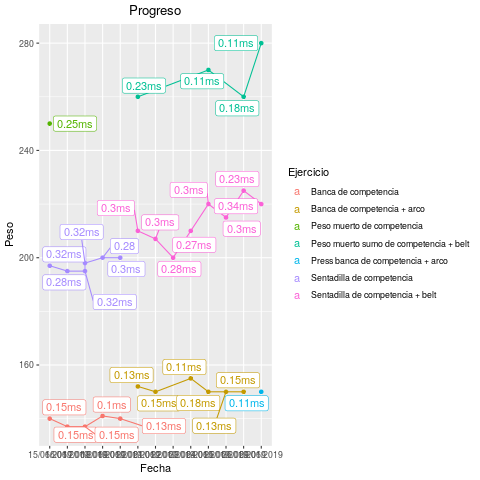
\includegraphics[width=.9\linewidth]{tmp.png}
\end{center}
\end{document}
